\documentclass[12pt, oneside]{article}   	% use "amsart" instead of "article" for AMSLaTeX format
\usepackage{geometry}                		% See geometry.pdf to learn the layout options. There are lots.
\geometry{letterpaper}                   		% ... or a4paper or a5paper or ... 
%\geometry{landscape}                		% Activate for rotated page geometry
%\usepackage[parfill]{parskip}    		% Activate to begin paragraphs with an empty line rather than an indent
\usepackage{graphicx}				% Use pdf, png, jpg, or eps§ with pdflatex; use eps in DVI mode
								% TeX will automatically convert eps --> pdf in pdflatex		
\usepackage{amssymb}

%SetFonts

%SetFonts


\title{Lab Write-Up Guide}
\author{Mark Peever\\ \texttt{mpeever@gmail.com}}
\date{2025-09-03}	

\begin{document}
\maketitle

\section{Overview}
There are several experiments (labs) in our textbook. When we complete those labs, either at home or in class, we need to record our experiment carefully to ensure our science is verifiable, falsifiable, and repeatable. 

There are some points to bear in mind for our lab write-ups:
\begin{enumerate}
\item the difference between a repeatable lab and an unrepeatable lab is organization
\item we want to gather both \emph{qualitative} and \emph{quantitative} data whenever possible
\item \emph{quantitative} (\emph{i.e.} numerical) data is much more valuable than qualitative data for repeatability
\item a picture is worth $10^{3}$ words
\end{enumerate}

\section{Template}
Your lab report should contain the following sections:

\subsection{Overview}
This should be a short paragraph laying out the purpose of the lab: what are you trying to demonstrate, prove, or test?

\subsection{Equipment List}
This doesn't have to be a fastidious list: we don't need to know how many pencils you used! We mainly want to know what pieces we'd need to gather to repeat your experiment. The list in the textbook should be a good guide.

\subsection{Procedure}
The idea here is to make the lab reproducible: the steps can be a short \emph{pr\'{e}cis} of the steps given in the text book.

\subsection{Observations and Data}
This is the most important part: it's where you record your observations.

This is important: we will always bias for numbers when possible.
An observation like ``the liquid turned blue" is useful, but it's not as repeatable as something like, ``$12 mg$ of Na fell out of solution."
The more precisely we can record our data, the more carefully we can compare our data with repeated experiments.

Whenever possible, we should record numbers in Tables: that helps us organize our observations.
If there is a repeated measurement (as there is in Experiment 1.4), we should look for a way to make a \emph{graph} of that data.

So, for example, in Experiment 1.4\footnote{Page 29 of our textbook}, we could come up with a table to record the measurements of each liquid like Table \ref{table:densitySamples} (page \pageref{table:densitySamples} ).

\begin{table}[p]
\centering
\begin{tabular}[b]{l | l| l}
\hline
Liquid & Volume & Mass \\
\hline
water                & $50mL$   & \makebox[2in]{\enspace\hrulefill} g \\
vegetable oil     & $50mL$   & \makebox[2in]{\enspace\hrulefill} g \\
maple syrup      & $50mL$   & \makebox[2in]{\enspace\hrulefill} g \\
\end{tabular}
\caption{Measured volumes and masses of various liquids}
\label{table:densitySamples}
\end{table}

In this example, a graph doesn't make a lot of sense. But if we were to look at something like the density of a liquid as we increase its temperature, we might be able to come up with a table that looks something like Table \ref{table:sampleTable} (page \pageref{table:sampleTable}).

\begin{table}[p]
\centering
\begin{tabular}[b]{l | l| l}
\hline
Temperature & Volume & Mass \\
\hline
$10^{\circ} C$ & $50mL$   & $12 g$ \\
$20^{\circ} C$ & $60mL$   & $12 g$ \\
$30^{\circ} C$ & $70mL$   & $12 g$ \\
$40^{\circ} C$ & $78mL$   & $12 g$ \\
\end{tabular}
\caption{Measured volumes of $12g$ of [some liquid] a various temperatures}
\label{table:sampleTable}
\end{table}

Now, \emph{this} would be something we could graph!\footnote{I get very excited when we can come up with a graph of our data.}

When we draw a graph, our \emph{controlled} measurement is horizontal, our \emph{resulting} measurement is vertical.
So in this example, we might come up with a graph like Figure \ref{figure:sampleChart} (page  \pageref{figure:sampleChart}).\footnote{Notice I don't make a ``Wall Street ticker tape" graph. There aren't line segments between each pair of data points.}

\begin{figure}[p]
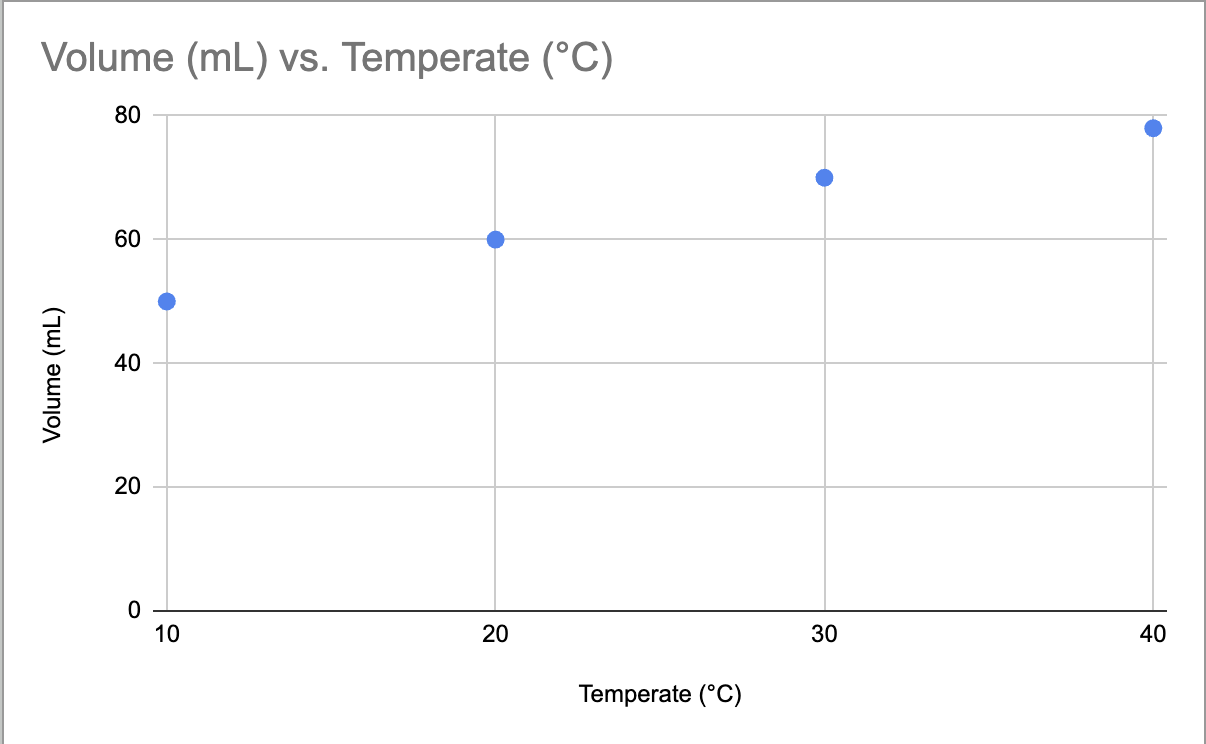
\includegraphics[scale=0.75]{Sample_Chem_Chart.png}
 \caption{Sample Chart}
 \label{figure:sampleChart}
 \end{figure}  

Remember, a picture is worth $10^3$ words, so we always look for opportunities to include graphs.


\subsection{Calculations}
If you have collected a whole lot of numerical data, here is a good place to show some math. Don't show all your work, but show an example for each row in your table data. For example, if you're calculating densities, show one density calculation ($\rho = \frac{m}{V}$), then show only the results for all the others.\footnote{This section will take some practice to get right.}

\subsection{Conclusion}
The conclusion is the ``so what?" of your experiment. What did you find? It's a place to put in what you discovered.

If you have numerical data you might put an equation here to describe it. In our example, you might present a formula that [seems to] match the graph we found: something like:\\  $$ V = (1 \frac{mL}{^{\circ}C}) T + 40mL $$

Here's where you'd also mention problems, and possible explanations. For example, in Experiment 1.4 you might mention that you measured densities on a particularly hot (or cold) day, so perhaps your numbers are lower than expected.

Remember significant figures! The significant figures from your measurements should be matched in whatever formulae and/or equations you have in your conclusion. 

\section{Final Notes}
\begin{itemize}
\item At least for the first few labs, we'll just write them up on looseleaf and turn them in like assignments.\footnote{I'd love to get proper lab books, but it'll be easier to manage our labs if we just use looseleaf.}
\item All labs are to be hand-written in pencil.
\item Keep lab write-ups to a page or two: these can easily get out of hand, but brevity is important.
\end{itemize}


\end{document}  